\chapter{Measurement of Encrypted Traffic} \label{chap:measurement-of-encrypted-traffic}

\begin{chapintro}

The application flow monitoring relies heavily on the ability to observe and process data from the application layer. However, users and companies are becoming more privacy conscious, and the use of encryption is steadily increasing. This chapter presents an overview of current approaches for the classification and analysis of encrypted traffic. The contribution of our work is four-fold. First, we describe several of the most widely used encryption protocols to show their packet structure and standard behaviour in a network. This information forms the basis of all classification protocols which use either a specific packet structure or a communication pattern to identify the protocol. Second, we investigate what information is provided by these encryption protocols. Most protocols negotiate encryption algorithms in clear-text, these data can be monitored, e.g., to reveal the use of weak ciphers. Third, we describe how the structure of encryption protocols can be used to detect these protocols in a network. Traffic classification algorithms using such information are presented, and we describe several open-source tools which implement these algorithms. Fourth, we provide an extensive survey of behaviour-based methods for encrypted traffic classification. We show that surprisingly detailed information can be obtained using these methods. In specific cases, even the content of the encrypted connection can be established.

The article included in this chapter is~\cite{Velan-2015-Survey}.

The organisation of this chapter is as follows:
\begin{itemize}
  \item Section~\ref{sec:enc-motivation} provides motivation for this chapter and defines its goals.
  \item Section~\ref{sec:traffic-description} explains the principles of several widely used encryption protocols.
  \item Section~\ref{sec:extraction} describes what information can be obtained from encrypted traffic using specific knowledge of the encryption protocols.
  \item Section~\ref{sec:taxonomy} describes the traffic classification taxonomy used in this chapter.
  \item Section~\ref{sec:payload-classification} describes traffic classification methods based on specific knowledge of encryption protocols.
  \item Section~\ref{sec:detection} surveys papers on the classification of encrypted traffic using statistical and behavioural methods.
  \item Section~\ref{sec:enc-conclusions} concludes the chapter and provides directions for future research.
\end{itemize}

\end{chapintro}

\newpage

\section{Motivation and Goals}\label{sec:enc-motivation}

% Motivation
Network visibility is becoming a necessity in current networks. Security, traffic provisioning, and failure detection are the prime reasons to deploy traffic measurement. Yet, measurement has other uses, and new ones are still being discovered. For instance, application performance can be measured using the data from the application layer. Information about certain applications can also be used to detect attacks and intrusions on the application level. In contrast to this, the need for protection of transmitted data and user privacy is rapidly increasing. It is for this reason that the encryption of transmitted data is increasingly used. The ratio of encrypted traffic has recently been rising steeply as common Internet services become protected~\cite{Sandvine-2014-Global}. This change poses a challenge to currently used methods for traffic measurement, for which the identification and analysis of network traffic become increasingly difficult.

Before any further analysis of encrypted network traffic can be done, the traffic needs to be identified. Statistical and behaviour-based application identification methods are less affected by encryption than deep packet inspection methods. Therefore, a lot of attention has been given to these methods, which are also considered to be privacy-conscious. However, information can even be extracted from encrypted connections, mainly from the session's initiation.

% Goal
The goal of this chapter is to provide a comprehensive overview of methods for classifying and analysing encrypted traffic. To the best of our knowledge, this is the first work which comprehensively summarises available approaches for encrypted traffic classification and analysis. Although there has been a lot of research on traffic classification in the past decade~\cite{Dainotti-2012-Issues, Nguyen-2008-Survey, Zhang-2009-State, Callado-2009-Survey, Finsterbusch-2014-Survey}, most of the existing surveys do not explicitly consider research which targets encrypted traffic. A recent survey by Cao et al.~\cite{Cao-2014-Survey} describes the fundamentals of encrypted traffic classification. It briefly introduces recent advances and challenges in this field. However, the survey covers only a few methods of traffic classification and does not provide any comparison or assessment of these methods. Moreover, while traffic classification is an important part of network monitoring, there are other methods for analysing encrypted traffic which need to be taken into consideration. 

To achieve this goal, we have produced a survey of methods for classifying and analysing encrypted traffic in journals, conference papers, proceedings of specialised workshops, and technical reports. We studied works presented in selected computer science journals, mainly the Communications Surveys \& Tutorials, Computer Networks, International Journal of Network Management, and Transactions on Network and Service Management. We also surveyed international conferences such as IMC, PAM, CISDA, CNSM, IM, and NOMS over the period 2005-2014. Other methods were found in references provided by the surveyed papers and in papers that referenced them.

Over the last decade, many statistical and machine learning algorithms have been applied to the problem of traffic classification. However, authors use different methodological datasets to evaluate their methods, and the results are therefore not directly comparable. Most of the methods use supervised or semi-supervised machine learning algorithms to classify flows and even determine the application protocol of the flow. Most methods target encryption protocols such as SSH, SSL/TLS, and encrypted BitTorrent. To describe and categorise the classification methods, we use the taxonomy of Khalife et al.~\cite{Khalife-2014-multilevel}. 


%%%%%%%%%%%%%%%%%%%%%%%%%%%%%%%%%%%%%%%% DESCRIPTION OF ENCRYPTION PROTOCOLS %%%%%%%%%%%%%%%%%%%%%%%%%%%%%%%%%%%%%


\section{A Description of Encryption Protocols} \label{sec:traffic-description}

This section provides a description of chosen encryption protocols. We selected the most widely used protocols to demonstrate the basic principles and show different approaches for secure data transport. Our choice of encryption protocols was also influenced by protocols which are the most commonly used in research of encrypted traffic classification. We shall describe IPsec, TLS, SSH, BitTorrent, and Skype protocols in this section. All these protocols provide confidentiality using encryption, and they usually offer authentication of communication peers, data integrity, replay protection, and non-repudiation. We shall describe the use of these protocols, their fundamental properties, the structure of encrypted packets, and the type of exchanged data. The information provided in this section will serve as the basis for rest of this chapter.

Almost all the presented encryption protocols can be divided into two main phases: the initialisation of the connection and the transport of encrypted data. The first phase can be further divided to an initial handshake, authentication, and a shared secret establishment. During the first phase, algorithm capabilities are usually exchanged, communication parties are authenticated, and secret keys are established. These keys are then used for encrypting transferred data in the second phase. This general protocol scheme is depicted in Figure~\ref{fig:protocols-scheme}, which, with minor modifications, can be applied to almost any protocol providing confidential data transfer.

\begin{figure}[!ht]
    \begin{center}
        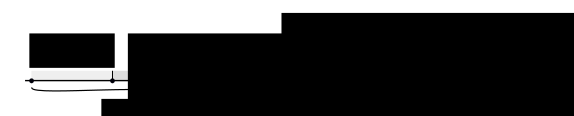
\includegraphics[width=0.9\textwidth]{figures/paper-encrypted/protocols_scheme}
        \caption{A General Scheme of Network Security Protocols.}
        \label{fig:protocols-scheme}
    \end{center}
\end{figure}

The protocols presented in this section are listed in order of their position in the ISO/OSI reference model~\cite{ISO7948-1}. IPsec protocol suite, which operates on the network layer is described first, followed by TLS and SSH protocols on the presentation layer. BitTorrent and Skype protocols represent the application layer, and they implement their own protocols for secure data transmission.


%%% IPSec %%%

\subsection{Internet Protocol Security}

Internet Protocol Security (IPsec) is a framework of open standards for ensuring authentication, encryption, and data integrity on the network layer. Due to its location on the network layer, IPsec can protect both the data within the packet and also L3 information (e.g., IP addresses) in each packet~\cite{SP-800-77}. The main advantage of using IPsec is securing the network connection without the necessity of modifying any application on the clients or servers. However, it provides less control and flexibility for protecting specific applications.

IPsec follows the general scheme depicted in Figure~\ref{fig:protocols-scheme}. The first phase is represented by the Internet Key Exchange Version 2 (IKEv2) protocol~\cite{rfc5996}. IPsec uses a UDP protocol on the port 500 through which all messages covering the initial handshake, the authentication, and the shared secret establishment run. Two protocols could be used in the second phase of IPsec: Authentication Header (AH) and Encapsulating Security Payload (ESP). In the initial version of IPsec, the ESP protocol providing data confidentiality did not include authentication, so ESP and AH were used together. Nowadays, the current version of ESP contains authentication, and AH has become less significant, although it is still used to authenticate portions of packets that ESP cannot manage.



\begin{figure}[!ht]
  \centering
  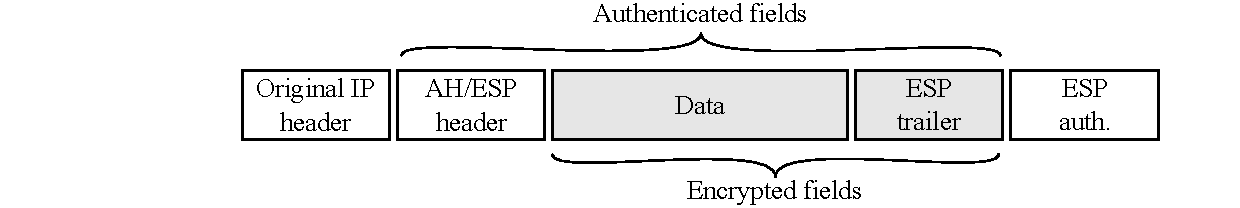
\includegraphics[width=0.9\textwidth]{figures/paper-encrypted/ipsec_transport_mode}
  \caption{The IPsec Packet Structure in the Transport Mode.}
  \label{fig:ipsec-transport-mode}
\end{figure}

\begin{figure}[!ht]
  \centering
  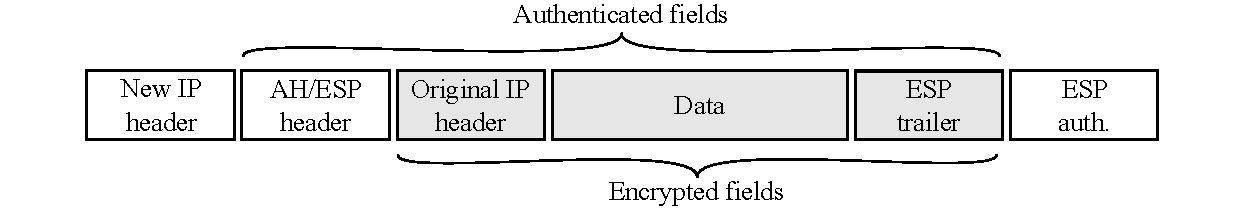
\includegraphics[width=0.9\textwidth]{figures/paper-encrypted/ipsec_tunnel_mode}
  \caption{The IPsec Packet Structure in the Tunnel Mode.}
  \label{fig:ipsec-tunnel-mode}
\end{figure}

The ESP protocol is the main protocol of IPsec. It provides data confidentiality, origin authentication, connectionless integrity, an anti-replay service, and limited traffic flow confidentiality~\cite{rfc4303}. ESP adds a header and a trailer to each transferred packet, see Figures~\ref{fig:ipsec-transport-mode} and~\ref{fig:ipsec-tunnel-mode}, placed according to the transport mode used. The ESP and AH protocols can operate in two modes: \textit{transport} and \textit{tunnel}. In the \textit{tunnel} mode, a new IP header is created for each packet with endpoints of the tunnel as the source and destination addresses; the original IP header is used in the \textit{transport} mode.



%%% TLS %%%

\subsection{Transport Layer Security}
Transport Layer Security (TLS)~\cite{rfc5246} is based on the Secure Sockets Layer version 3 (SSLv3) protocol~\cite{rfc6101} and provides transport level security directly on top of the TCP protocol. Specifically, it provides confidentiality, data integrity, non-repudiation, replay protection, and authentication through digital certificates. The TLS is currently one of the most common protocols for securing network communication. It is mainly used for securing HTTP, FTP, SMTP sessions, as well as for Virtual Private Networks or Voice over Internet Protocol (VoIP). The protocol design is layered and consists of different sub-protocols, as well as configurable and replaceable cryptographic algorithms~\cite{tls-thesis}.

The main part of TLS is the Record Protocol~\cite{rfc5246}, which acts as an envelope for application data as well as TLS messages. In the case of the application data, the Record Protocol is responsible for dividing the data into optionally compressed fragments. The addition of fragments to the record is complemented by Message Authentication Code (MAC). For more details, see Figure~\ref{fig:tls-record}. Depending on the selected security algorithms, a fragment and MAC are encrypted together and sent as one TLS record. A packet may contain more than one record to avoid sending multiple short packets.

\begin{figure}[!ht]
    \begin{center}
        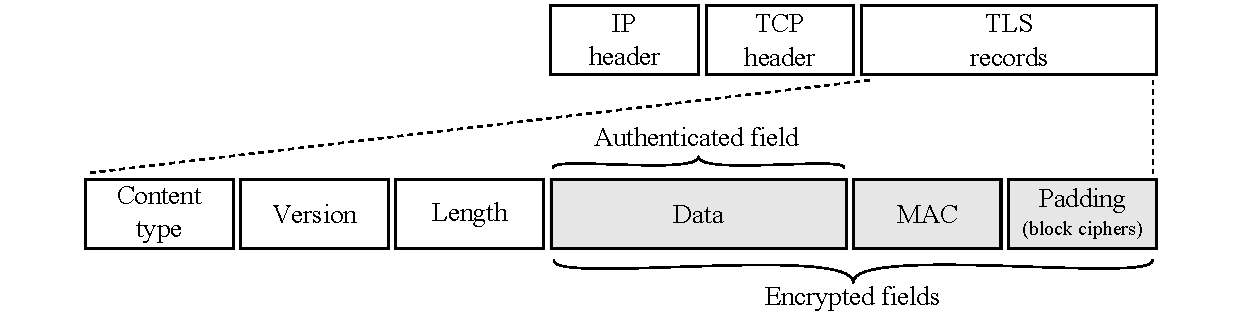
\includegraphics[width=0.9\textwidth]{figures/paper-encrypted/tls_record}
        \caption{The TLS Record Packet Format.} 
        \label{fig:tls-record}
    \end{center}
\end{figure}

During the first phase of a TLS connection, communicating parties are usually authenticated (more often we can see only server authentication) using an X.509 certificate chain~\cite{rfc5280}, as shown in the general scheme in Figure~\ref{fig:protocols-scheme}. Alternatively, a previous connection can be resumed without authentication. TLS messages exchanged during this phase are unencrypted and do not contain MAC until the shared keys are established and confirmed. In the second phase, these keys are used directly by the Record Protocol, which is based on the selected algorithms ensuring communication security.

%%% SSH %%%

\subsection{Secure Shell Protocol}
In a similar fashion to the TLS protocol, the Secure Shell (SSH) protocol~\cite{rfc4253} exists as a separate application on top of TCP. This protocol uses a client-server model where the server usually listens to the TCP port 22. SSH was originally designed to provide remote login access to replace unsecured Telnet connections. Nowadays, it can be used not only for remote login and a shell, but also to allow file transfers using the associated SSH File Transfer Protocol (SFTP)~\cite{sftp-draft} and a Secure Copy (SCP)~\cite{scp-description} protocol, or by Virtual Private Networks (VPN). The SSH protocol provides user and server authentication, data confidentiality and integrity, and optional compression.

\begin{figure}[!ht]
    \begin{center}
        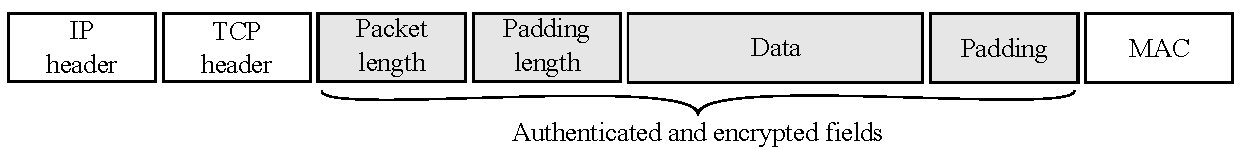
\includegraphics[width=0.9\textwidth]{figures/paper-encrypted/ssh_packet}
        \caption{The SSH Protocol Packet Format.} 
        \label{fig:ssh-packet}
    \end{center}
\end{figure}

SSH consists of three protocols, of which the most important is the Transport Layer Protocol, which provides the establishment of the whole connection and its management. It defines the SSH packet structure, which is depicted in Figure~\ref{fig:ssh-packet}. The MAC code is computed on a plaintext payload together with the packet length, the padding, and a continuously incremented sequence number not present in the packet itself. Other SSH protocols are the User Authentication Protocol and the Connection Protocol for multiplexing multiple logical communication channels~\cite{ssh-basics}.

Each SSH connection passes through the same phases which were depicted in Figure~\ref{fig:protocols-scheme}. In the first phase, a TCP connection is established, and information about preferred algorithms is exchanged. During authentication, the server sends its public key which must be verified by the client (using a certification authority or manually through a different channel). The shared keys are subsequently established and confirmed. All following packets are then encrypted and authenticated.


%%% Bittorent %%%

\subsection{BitTorrent}
BitTorrent~\cite{bittorrent-specification} is an application protocol based on the principle of peer-to-peer network communication for sharing large amounts of data over the Internet. Originally, the protocol did not ensure any type of network communication security. Once the popularity of this protocol increased, some Internet Service Providers (ISP) started to limit this type of traffic. As a response to this, the Message Stream Encryption (MSE) algorithm~\cite{mse-specification}, also known as Protocol Encryption (PE), was introduced. It serves as an obfuscation algorithm to make BitTorrent traffic identification more difficult. In addition to obfuscation, the mechanism also ensures some level of confidentiality and authentication for communicating peers.

The MSE protocol specification~\cite{mse-specification} describes MSE as a transparent wrapper for bidirectional data streams over TCP which prevents passive eavesdropping and thus protocol content identification. MSE is also designed to provide limited protection against active man-in-the-middle attacks and port scanning by requiring a weak shared secret to complete the handshake. The major design goal was payload and protocol obfuscation, not peer authentication or data integrity. Thus, it does not offer protection against adversaries which already know the necessary data to establish connections (that is the IP/port/shared secret/payload protocol).

The first general phase of the MSE protocol follows a TCP three-way handshake and starts with a newly generated Diffie-Hellman (DH) public key exchange (together with random data padding for better obfuscation). The shared key is computed by the DH key and combined with hashed information about the requested data which acts as a pre-shared secret. The packet's payload is completely encrypted by an RC4 stream cipher after successfully confirming the shared key.

%%% Skype %%%

\subsection{Skype}
Skype~\cite{skype-web} is a peer-to-peer based VoIP application providing not only video chat and voice calls, but also an instant messaging and file exchange service. As the protocol used is not publicly known, it is not possible to accurately describe its specific details. The main reason for this is network data obfuscation to make the detection of Skype traffic more difficult, which is similar to the BitTorrent protocol.

The Skype protocol operates over both UDP and TCP protocols depending on network characteristics. If the network has no restrictions, the application usually sends data traffic over UDP and the signalling traffic over TCP~\cite{skype-hunter}. If UDP cannot be used (for example a firewall prevents users from using such a protocol), Skype sends both the signalling and the data traffic over TCP. When TCP is used, the connection is usually established over port 80 or 443, which masks Skype traffic as standard web traffic.

Skype uses the TLS protocol over the TCP port 443 and a proprietary protocol over port 80~\cite{skype-hunter} for securing and obfuscating generated traffic of each communicating peer. TLS is also used in communication with other Voice over IP solutions, where it is used for protecting Session Initiation Protocol (SIP) messages~\cite{skype-requirements}. Skype uses a proprietary protocol for communication over UDP. To offer a reliable connection, UDP packets contain an unencrypted header with a frame ID number and function mode fields. The encryption in UDP connections is used only for obfuscation and not for confidentiality; therefore, there is no generated shared secret, only a proprietary key expansion algorithm. UDP connections do not follow the general scheme in Figure~\ref{fig:protocols-scheme} because encrypted data are directly transferred without an initialisation phase.

%%%%%%%%%%%%%%%%%%%%%%%%%%%%%%%%%% Information Extraction from Encrypted Traffic %%%%%%%%%%%%%%%%%%%%%%%%%%%%%%%%%


\section{Information Extraction from Encrypted Traffic}\label{sec:extraction}


Network monitoring is one of the main pillars of network security. If the appropriate data are collected, it is possible to detect network attacks and trace attackers, detect security policy violations and monitor network applications performance. If encrypted traffic is used, the possibility of information extraction is significantly limited. Nevertheless, it is possible to obtain some information from this traffic, primarily from the unencrypted initialisation phase, but also from the encrypted transport phase. This section begins with a description of the initialisation phase, which is then followed by a description of methods which use traffic feature analysis to gain information from the transport phase.


\subsection{The Unencrypted Initialization Phase}

Almost all network protocols ensure secure data transfer by means of encryption containing an unencrypted initialisation phase, as depicted in Figure~\ref{fig:protocols-scheme}. Because the data exchanged at this stage are not encrypted, they can be easily extracted and used for monitoring of network traffic. Generally, two types of information common to most protocols can be extracted during this phase. The first type covers the connection itself, and its properties exchanged in the initial handshake. The second type covers communicating peers' identifiers which are exchanged in the authentication phase.

During the initial handshake, parameters of a connection are negotiated, such as which cipher suite and protocol version is used. This dynamic setting of the connection properties enables backward compatibility for different versions of software or is used to set a different level of security based on established security policies. Some examples of this are data authentication and compression in addition to the encryption itself. The list of possible identifications, with references to algorithm specification for IPsec, TLS, SSH, and other protocols, can be found in IANA Protocol Registries~\cite{iana-protocol-registries}. All of this information can be used for proper connection characterisation and correct parsing of other packets in the rest of the connection.

One interesting use of the information from the initial handshake is presented by client fingerprinting based on the provided cipher-suites. A large amount of cipher-suites types exists, which usually are not all implemented by the client's applications. Therefore, each application specifies the supported cipher-suites and also the order of their preference during the initial handshake. This makes it possible to passively distinguish specific operating systems, web browsers, and other applications, together with their versions, based only on the cipher-suites which they use. An example of such client fingerprinting, based on the SSL/TLS initial handshake, is presented by applications from SSL Labs~\cite{qualys-ssl-fingerprinting} and p0f module~\cite{p0f-ssl-fingerprint}.

The authentication phase represents the second source of information which can be easily extracted from secured network traffic. Unique identifiers of one or both communicating peers, optionally supplemented by additional data about them, are exchanged during this phase. For example, in the authentication phase of the SSH protocol, the server sends its public key to the user. The user must validate the key and verify that the server knows the appropriate private key~\cite{rfc4253}. Since this information is almost unique for each SSH server, it is possible to detect server changes or man-in-the-middle attacks on them by passive network traffic monitoring. 

A very good example of extracting information from communication peers is demonstrated by monitoring the authentication phase of the SSL/TLS protocol. The server, and optionally even the client, send their X.509 certificates~\cite{rfc5280} to each other to verify their identities in this phase. This certificate contains a public key signed by the certification authority which is supplemented with information about the peer and issuer. A more detailed content of such certificates is shown in Figure~\ref{fig:certificates-contents}.

\begin{figure}[!ht]
    \begin{center}
        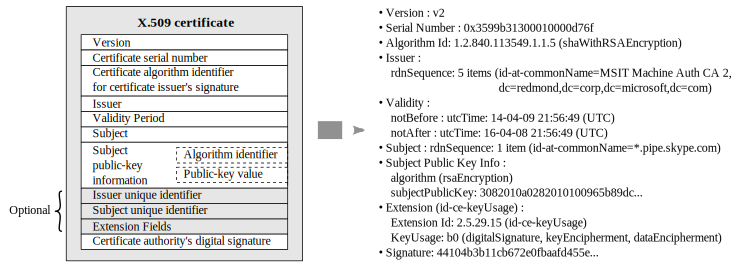
\includegraphics[width=0.9\linewidth]{figures/paper-encrypted/certificate}
        \caption{Example of Skype X.509 Certificate.}
        \label{fig:certificates-contents}
    \end{center}
\end{figure}

Passive monitoring of certificates enables not only the identification of communicating peers but also the ability to check whether these certificates are valid and contain proper security algorithms to fulfil local security policies. SSL/TLS certificate properties were studied by Holz et al.~\cite{Holz-2011-SSL} who revealed a great number of invalid certificates some of which were shared between a large number of hosts. The work of Holz et al. was followed by Durumeric et al.~\cite{Durumeric-2013-Analysis} who focused mainly on assessing certification authorities. Certificate monitoring can also be used to detect malicious software trying to hide its activities by connecting with their command and controls centres using the SSL/TLS protocol~\cite{ssl-certificates-blacklist}.

Even though information extraction from encrypted traffic is not a computationally intensive process, it can provide valuable information. For example, extracting the Server Name Indication (SNI)~\cite{rfc4366} can be used by a home router's firewall to filter traffic. The unencrypted initialisation phase is often used to recognise encrypted traffic, and the authentication information might be utilised to detect and prevent man-in-the-middle attacks on a network-wide level.

\subsection{The Encrypted Data Transport Phase}

Information about network traffic can be extracted from encrypted data which is transported between communicating parties. Packets exchanged during the transport phase usually contain only information about the packet itself, such as the length and the authentication field which are not useful for monitoring network traffic. Nevertheless, two methods to obtain more suitable data do exist.

The first method uses direct traffic decryption, which is possible to perform only if the shared secret of the connection is known. Therefore, decryption can be used in networks on the servers' side where organisations know the private key of the connected server. However, such decryption would be impossible if algorithms which ensure forward secrecy~\cite{Huang-2014-tls-forward-secrecy} were used. 

The second method is based on the extraction of traffic features. An example of such an analysis is presented by Miller et al.~\cite{Miller-2014-https-decrypt} who monitor the size of TLS encrypted packet sequences. Based on their data, together with various predictive models, they are able to identify a specific web page and deduce its content even though the traffic is encrypted. A similar approach was also used by Koch and Rodosek~\cite{Koch-2010-Command} for analysing SSH traffic. Another example of using traffic features is the work by Hellemons et al.~\cite{hellmons-2012-sshcure}, which focused on intrusion detection in SSH traffic. Encrypted traffic features could also be used for classifying encrypted traffic, which is described in Section~\ref{sec:detection}.


%%%%%%%%%%%%%%%%%%%%%%%%%%%%%%%%%%% Taxonomy for Traffic Classification Methods %%%%%%%%%%%%%%%%%%%%%%%%%%%%%%%%%%


\section{A Taxonomy for Traffic Classification Methods} \label{sec:taxonomy}

The first step in analysing network traffic is identifying the type of the measured traffic. Network traffic classification methods are used for this purpose based on the knowledge of the protocol packet structure, communication patterns, or a combination of both.The recognition of the TLS protocol, described in Section~\ref{sec:traffic-description}, may be seen as an example of this. This protocol can be identified based on the knowledge of the packet structure, especially the unencrypted packet parts such as the content type, version, and length. Similarly, the protocol can be identified by analysing its behaviour, e.g., the knowledge of a number and an approximate size of packets sent during the unencrypted initialisation phase.

To present the current state of research on encrypted traffic classification in a comprehensive manner, we use a taxonomy of classification methods. We choose the multilevel taxonomy by Khalife et al.~\cite{Khalife-2014-multilevel}, which provides a detailed categorisation of traffic classification methods. This taxonomy is uniquely descriptive and allows us to efficiently categorise all our surveyed classification methods. Figure~\ref{fig:taxonomy} shows an overview of the taxonomy levels. On the topmost level, the authors distinguish between classification input, technique, and output. The input determines the traffic's characteristics, which are used for classification (e.g., packets or flows). The technique describes the core of the classification method, which may be, among others, payload inspection, a statistical method, or a machine learning method. The output then describes how the traffic objects (packets or flows) map to traffic classes (application types or application protocols). The traffic classes are of different granularity. Some methods allow identification of application protocols (e.g., HTTP), and some are more fine-grained to detect, for example, a Google search or a Facebook chat.

\begin{figure}[!ht]
    \begin{center}
        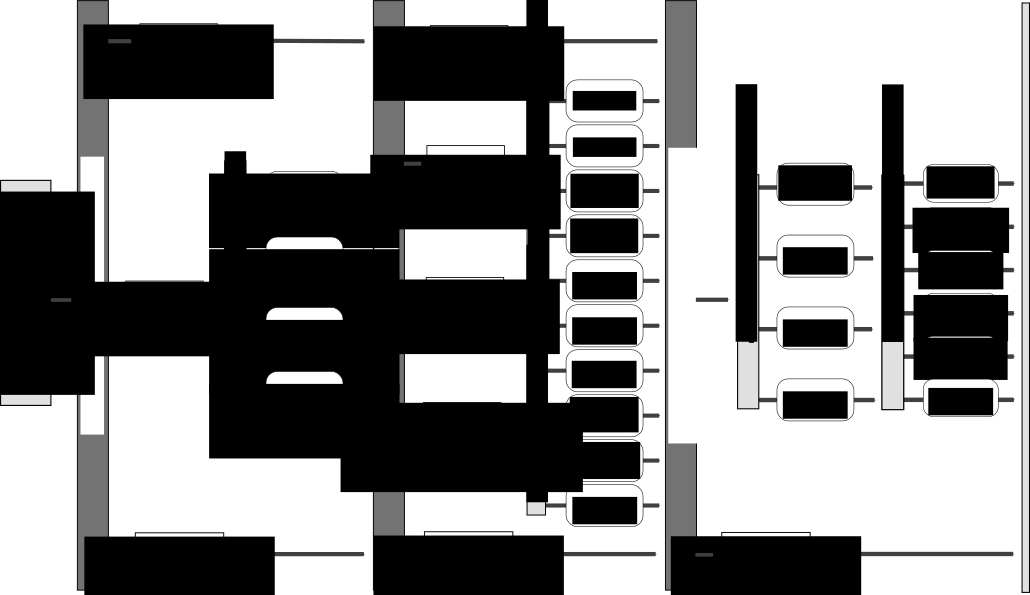
\includegraphics[width=\textwidth]{figures/paper-encrypted/taxonomy}
        \caption{A Multilevel Taxonomy of Traffic Classification Methods~\cite{Khalife-2014-multilevel}.} 
        \label{fig:taxonomy}
    \end{center}
\end{figure}

\begin{table}[!ht]
    \centering
    \small
    \renewcommand{\arraystretch}{1.05}
    \begin{tabularx}{\textwidth}{c|l|X} \hline
        \multicolumn{3}{ c }{\textbf{Classification Input}} \\ \hline \hline
        \multicolumn{2}{ c| }{\textit{Traffic Payload}} & use of application data \\ \hline
        \multirow{3}{*}{\parbox[c]{3.6cm}{\centering\textit{Traffic Properties}\\ (Measurement Level)}} & Host Community & graph metrics (diameter, connection degree) \\
        & Host & number of connections, opened ports \\
        & Flow & flow size, flow duration \\
        & Packet & packet sizes, inter-arrival times \\ \hline
        \multicolumn{2}{ c| }{\textit{Hybrid \& Miscellaneous}} & combination of inputs, external knowledge \\ \hline
    \end{tabularx}
    \smallskip
    \caption{Classification Input Level.}
    \label{tab:classification-input}
\end{table}

\begin{table}[!ht]
    \centering
    \small
    \renewcommand{\arraystretch}{1.05}
    \newcommand{\classificationsize}{2.7cm}
    \begin{tabularx}{\textwidth}{c|l|X} \hline
        \multicolumn{3}{ c }{\textbf{Classification Technique}} \\ \hline \hline
        \multicolumn{2}{ c| }{\textit{Payload Inspection}} & DPI, examination of first N bytes \\ \hline
        \multirow{3}{*}{\parbox[c]{\classificationsize}{\centering\textit{Graphical\\ Techniques}}} & Graphlets & relationship between features (ports, addresses) \\
        & Motifs & patterns of communication \\
        & Social Networks & graph of communication \\ \hline
        \multirow{3}{*}{\parbox[c]{\classificationsize}{\centering\textit{Statistical\\ Method}}} & Basic Statistical & probability density functions of e.g., packet sizes \\
        & Heuristics & port-based classification \\
        & Profiles & host profiling, usage of packet sizes and direction \\ \hline
        \multirow{3}{*}{\parbox[c]{\classificationsize}{\centering\textit{Machine Learning\\ Algorithm}}} & Supervised & Hidden Markov Models, Naive Bayes, $k$-nearest neighbour, support vector machine \\
        & Non-Supervised & clustering of unlabeled traffic, \mbox{$k$-nearest} neighbour \\
        & Semi-Supervised & clustering of mixed traffic, \mbox{$k$-nearest} neighbour  \\
        & \parbox[c]{3.5cm}{Reinforcement Learning} & - \\ \hline
        \multicolumn{2}{ c| }{\textit{Hybrid \& Miscellaneous}} & combination of methods, external knowledge \\ \hline
    \end{tabularx}
    \smallskip
    \caption{Classification Technique Level.}
    \label{tab:classification-technique}
\end{table}

\begin{table}[!ht]
    \centering
    \small
    \renewcommand{\arraystretch}{1.05}
    \begin{tabularx}{\textwidth}{c|X} \hline
        \multicolumn{2}{ c }{\textbf{Classification Output}} \\ \hline \hline
        \multicolumn{2}{ c }{\textbf{Traffic Objects}} \\ \hline
        Host Community & host community is assigned a class, e.g., community of HTTP servers \\
        Host & host is assigned a class \\
        Flow & flow is assigned a class \\
        Packets & packet is assigned a class \\ \hline \hline
        \multicolumn{2}{ c }{\textbf{Traffic Classes}} \\ \hline
        Traffic Cluster &  bulk or small transactions\\
        Application Type & game, browsing, chat \\
        Application Protocol & HTTP, HTTPS, FTP \\
        Application Software & client software such as Mail client, FTP client or web browser \\
        Fine-Grained & Skype voice call, Google search, Facebook chat \\
        Anomaly & port scan, brute-force attack \\ \hline \hline
        Hybrid \& Miscellaneous & combination of outputs or classes, external knowledge \\ \hline
    \end{tabularx}
    \smallskip
    \caption{Classification Output Level.}
    \label{tab:classification-output}
\end{table}

Tables~\ref{tab:classification-input}, \ref{tab:classification-technique}, and \ref{tab:classification-output} provide examples for each of the input, technique, and output category. The input and technique tables have the most general categories in the left column, some of which are divided into more specific subcategories. The classification output table is divided horizontally into traffic objects and classes. The objects describe what is being classified, in other words, whether it is each packet, whole flow or a host. Traffic classes describe the type of classification being performed by a specific algorithm.


%%%%%%%%%%%%%%%%%%%%%% Payload-Based Traffic Classification Techniques for Encrypted Traffic %%%%%%%%%%%%%%%%%%%%%


\section{Payload-Based Traffic Classification Techniques for Encrypted Traffic}\label{sec:payload-classification}


Almost every network traffic encryption protocol has a specific packet format that differs from others, as was described in Section~\ref{sec:traffic-description}. Thus, with knowledge of these formats, it is possible to distinguish and identify individual protocols by inspecting the packet payload. It is for this purpose that string or regular expression matching algorithms are used together with specific protocol patterns. Some examples of contemporary classification tools which use payload inspection are discussed in more detail in the first part of this section. The second part presents current research papers which focus on comparing these tools in terms of their performance and success rate.


\subsection{Payload-Based Classification Tools}

Most network traffic classification tools aim to recognise all network protocols and not only the encrypted ones. The following examples represent the most widely used tools for classifying network traffic. Most of these tools are also able to distinguish specific network applications, mainly in unencrypted traffic. In terms of the taxonomy, these tools mostly use the \textit{Payload Inspection} technique on the \textit{Traffic Payload} classification input to map \textit{Flows} to \textit{Application Protocols}.

\textit{PACE}~\cite{pace} is a commercial classification library written in C, which uses pattern matching augmented by heuristics, behavioural, and statistical analysis. In addition to standard protocol and application recognition, it is able to identify obfuscated protocols such as BitTorrent or Skype. According to its website, PACE is able to identify thousands of network applications and protocols.

\textit{Cisco Network-Based Application Recognition (NBAR)}~\cite{CiscoSystems--Network} is another example of a commercial tool for classifying network traffic. This tool is primarily used on Cisco routers for quality and security purposes. According to its authors, NBAR is also able to recognise stateful protocols as well as non-TCP and non-UDP IP protocols.

\textit{nDPI}~\cite{Deri-2014-nDPI} is an open-source classifier forked from the (currently closed) project OpenDPI, which was in turn derived from PACE. nDPI analyses at most eight packets from each connection for classifying traffic, however, each packet is examined separately. If the connection contains multiple matches, then the most detailed match is returned. For encrypted traffic recognition, nDPI contains only a SSL decoder that extracts the hostname from the server certificate. By using these names, nDPI is able to identify specific network applications.

\textit{Libprotoident}~\cite{Alcock-2012-libprotoident} is an open-source C library for classifying traffic. In contrast to the previous tools, Libprotoident inspects only the first four bytes of a packet payload for each direction. This makes it much faster but reduces its detection accuracy. The classification uses a combined approach of pattern matching, payload size, port numbers, and IP matching.

\textit{L7-filter}~\cite{l7-filter} is an open-source classifier for Linux which is designed to classify traffic on the application layer. The initial phase of classification is based on non-payload data such as port numbers, IP protocol numbers, the number of transferred bytes, and so forth. Payload data are analysed with regular expressions during the second phase. One disadvantage of the l7-filter is that it contains a database with old patterns which was last updated in 2011.


\subsection{A Comparison of Classification Tools}
A comparison of the presented open-source tools was introduced by Finsterbusch et al.~\cite{Finsterbusch-2014-Survey}. They prepared a dataset containing the traffic of 14 different network protocols such as DNS, HTTP, BitTorrent, and SMTP(S) to compare the tools. Using this dataset, they measured classification accuracy, memory usage, CPU utilisation, and the number of packets required for proper classification. The comparison showed, amongst other results, that nDPI is not able to classify the BitTorrent protocol with more than a 43\,\% true positive rate, although it detects SSL/TLS with 100\,\% accuracy. The Libprotoident tool had the highest classification accuracy on the whole analysed traffic, and was able to classify DNS, HTTP, SIP, and e-mail protocols with 100\,\% accuracy. Libprotoident also needs the least number of packets on average for classifying real-time traffic. Based on the comparison by Finsterbusch et al., we can say that Libprotoident is the most appropriate tool for classifying payload-based traffic, although it is more CPU intensive than the other tools.

Another comparison of the tools was carried out by Bujlow et al.~\cite{Bujlow-2015-classification}. They compared all of the previously presented tools. They prepared a publicly available dataset for the comparison which contained encrypted and unencrypted network traffic from 17 application protocols, 25 network applications and 34 web services. Their results show that PACE and Libprotoident are the most accurate tools. Nevertheless, the Libprotoident tool was the only classifier able to identify all the encrypted protocols which were tested. Their results were generally very similar to those in the comparison by Finsterbusch et al.

In general, the payload-based classification tools utilise regular expression matching algorithms to identify the encrypted traffic. The main difference between the tools is how much data they need to examine and whether they need both directions of the connection for the classification.


%%%%%%%%%%%%%%%%%%%%%% Feature-Based Traffic Classification Techniques for Encrypted Traffic %%%%%%%%%%%%%%%%%%%%%


\section{Feature-Based Traffic Classification Techniques for Encrypted Traffic}\label{sec:detection}


This section surveys feature-based classification methods which specialise in encrypted traffic. These methods do not require any knowledge of the encryption protocol packet structure. Instead, they use specific protocol communication patterns to classify encrypted traffic. The methods are based on the specific protocol differences described in Section~\ref{sec:traffic-description}, such as packet and flow features of unencrypted initialisation or the encrypted data transport phase. This approach provides greater generalisation and allows these methods to work with new versions and types of encryption protocols without the modification of underlying algorithms.

The taxonomy specified in Section~\ref{sec:taxonomy} is used to describe the individual methods. Apart from the properties defined by the taxonomy, we also provide information about datasets used for evaluating these methods. This is especially important when additional evaluation is to be performed by other research groups to verify the results of the authors. While the taxonomy provides a traffic class for classifying the application protocol, this is sometimes too coarse for our purposes. Most classification methods identify not only the encryption protocol but also the underlying encrypted application protocol. As both cases belong to the application protocol traffic class, we provide further explanation in the description of each classification method.

A slight drawback of most flow-based classifiers is in performing the classification only after the flow has expired. This prevents the possibility of a real-time response, which has led several research groups to research real-time classification using flow-features. Their methods are also included with the others in Table~\ref{tab:method_categories} and differentiated by a column describing whether the classification is done in real-time or not.

Almost 250 discriminators (flow or packet features) are identified by Moore et al.~\cite{Moore-2005-Discriminators}, which can be used to classify flow records. The authors do not propose any specific classification method themselves, however, most of the classification algorithms use a subset of these discriminators for identifying traffic. In terms of the taxonomy, the authors provide a list of traffic features which are used to infer the category of the traffic's properties for the classification input.

Most of the feature-based traffic classification methods use statistical or machine learning methods. These methods are comprehensively described in \cite{Alpaydin-2010-Introduction}. A port-based classification was used in the past to associate applications with network connections, but the accuracy of this method is decreasing with the increased use of dynamic ports and applications evading firewalls. Despite the decreased accuracy, port numbers are often utilised as one of the packet features. Furthermore, port-based classification is still quite often used to establish a ground truth for traffic classification experiments.

For easier orientation, we present the surveyed papers grouped by the class of their traffic classification algorithm. Most of the papers employ Supervised Machine Learning Methods (Section~\ref{subsec:supervised}), Semi-Supervised Machine Learning Methods (Section~\ref{subsec:semisupervised}), and Basic Statistical Methods (Section~\ref{subsec:basic-statistical}). The rest combine more than one method and are therefore gathered in a Hybrid Methods category (Section~\ref{subsec:hybrid}). For each surveyed paper, we specify the classification technique, classification output, and the datasets used in the description of the classification process itself. Table~\ref{tab:method_categories} in Section~\ref{subsec:methods-summary} provides a summary of the papers with all of the mentioned properties properly categorized.

\subsection{Supervised Machine Learning Methods}\label{subsec:supervised}

Sun et al.~\cite{Sun-2010-Novel} propose a hybrid method for classifying encrypted traffic. First, the SSL/TLS protocol is recognised using a signature matching method. A Naive Bayes machine learning algorithm is then applied to identify the encrypted application protocol. The authors use a combination of public and private datasets to evaluate their method. Background traffic is taken from a public dataset, BitTorrent, eDonkey, HTTP, FTP, Thunder, and GRE application protocols. The signature based recognition of SSL/TLS protocols was tested on HTTPS, TOR, ICQ, and other protocols. The identification of the underlying protocol was tested only for TOR and HTTPS protocols.
% INPUT: packet payload, flows (8 features)
% TECHNIQUE: [payload inspection, supervised] (naive Bayes)
% OUTPUT: flows->application protocol (in SSL/TLS)
% dataset: public and private, real
% partial flow: no

Okada et al.~\cite{Okada-2011-Application} analysed changes in flow features due to encryption. They created a training dataset with HTTP, FTP, SSH, and SMTP application protocols encrypted using PPTP and IPsec tunnels. The authors assessed 49 flow features and analysed which of them are strongly correlated in normal and encrypted traffic. The correlated features were then used to infer functions which transform the features from normal to encrypted traffic. Therefore, standard classifiers can be used to classify the traffic after the transformation. The authors verified their method using several modifications of the Naive Bayesian classifier.
% INPUT: Flow
% TECHNIQUE: MLA->Supervised (Naive Bayes)
% OUTPUT: Flow->Application Protocol
% dataset: private, artificial
% partial flow: no

Arndt and Zincir-Heywood~\cite{Arndt-2011-Comparison} also concentrated on the classification of encrypted traffic and compared C4.5, $k$-means, and Multi-Objective Genetic Algorithm (MOGA) to this end. The classification of the SSH protocol was used as an example in their study. The authors focused on the accuracy and robustness of the algorithms. Stability was tested using three different public and private datasets for teaching and evaluating the methods. Multiple different flow export settings were tested as well. Altogether, 46 flow features were used in the evaluation, however, a different subset was used by each algorithm. The C4.5 algorithm provided the best robustness, although the MOGA had a very low false positive rate when used on the same dataset it was trained on. The C4.5 was recommended for forensic analysis by law enforcement since it is applicable to a variety of networks.
% INPUT: Flows
% TECHNIQUE: Supervised (C4.5, $k$-means, MOGA)
% OUTPUT: application protocol (SSH, non-SSH)
% dataset: private, public, real
% partial flow: no

% Summary of 4 Alshammari works:
Alshammari and Zincir-Heywood have published several papers~\cite{Alshammari-2009-Classifying, Alshammari-2007-flow, Alshammari-2009-Preliminary, Alshammari-2009-Machine, Alshammari-2010-Investigation, Alshammari-2011-Can} on traffic classification using various supervised machine learning methods. They focused on recognising SSH, Skype, and in one case, Gtalk traffic using flow features without port numbers, IP addresses, or payloads. A set of 22 flow features was mostly used, although in one case the authors selected the features using genetic programming. Public datasets are used as well as a private dataset generated on a testbed network. The ground truth for public datasets was gained from port numbers, and the private dataset included the payload and was labelled with a commercial packet classification tool. The following algorithms for traffic classification were compared: AdaBoost, RIPPER, Support Vector Machine (SVM), Naive Bayes, C4.5, and Genetic Programming.

Kumano et al.~\cite{Kumano-2014-Towards} investigated identification of real-time applications in encrypted traffic. IPsec and PPTP encryption were applied to the web, interactive and bulk transfer flows to create an evaluation dataset. C4.5 and SVM algorithms were utilised to classify the application on these datasets. The authors then tested the accuracy of the classification using a different number of packets from the start of the flows. They measured the impact of using fewer packets on the flow features and proposed using features which show the least change to classify applications at an early stage.
% INPUT: Flows
% TECHNIQUE: Supervised (C4.5, SVM)
% OUTPUT: Flow->application type
% dataset: private, artificial
% partial flow: 


\subsection{Semi-Supervised Machine Learning Methods}\label{subsec:semisupervised}

Bernaille and Teixeira~\cite{Bernaille-2007-Early} used traffic clustering to detect applications encrypted by SSL. Their method has three steps. First, they detected SSL connections using a clustering algorithm (Gaussian Mixture Model) on packet sizes and directions of initial packets of a connection. The first three packets and 35 clusters provide good accuracy in detecting SSL traffic. After the SSL traffic is identified, the first data packets of the connections are identified. The sizes of the data packets are used by a clustering algorithm to detect an underlying application in the third step. However, the packet sizes are modified in the last step to allow for encryption overhead. The evaluation of the proposed method is done on traffic traces from live networks and a manually generated packet trace. The datasets contain HTTP, POP3, FTP, BitTorrent and eDonkey application protocols encrypted using SSL. The authors also show that using a combination of clustering and port numbers to differentiate between applications in clusters provides better results than clustering alone.
% INPUT: packet
% TECHNIQUE: non-supervised, clustering (Gaussian Mixture Model)
% OUTPUT: flow->application protocol
% dataset: custom, real, published
% partial flow: yes

Maolini et al.~\cite{Maiolini-2009-Real} identify SSH traffic and determine transported application protocols, such as SCP, SFTP, and HTTP, using a $k$-means algorithm. Only three packet features are used: the direction, the number of bytes, and the timestamp of each packet. Their private datasets are created from artificial traffic and contain HTTP, FTP, POP3, and SSH protocols. Control packets such as TCP handshake, retransmitted packets, and ACK-only packets are removed from the statistics as they negatively affect the precision. Authors use only first 3-7 packets to achieve a real-time identification.

Backquet et al.~\cite{Bacquet-2009-Investigation, Bacquet-2011-Genetic} use a Multi-Objective Genetic Algorithm to select a flow feature subspace and parameters for a clustering algorithm which detects encrypted traffic. The second work employs a hierarchical $k$-means algorithm to increase the identification's accuracy. The authors evaluate both approaches on a private dataset captured at a university campus. SSH is used as a representative of encrypted traffic, and the ground truth is gained from the payload of the captured packets. Based on previous works, the authors argue that the feature selection and the number of clusters highly affect the overall accuracy. Therefore, the authors selected four objectives for the genetic algorithm: cluster cohesiveness, cluster separation, the number of clusters and the number of used flow features. The results show (a) that only 14 from a total of 38 flow features were used by the best-performing algorithm and (b) that using a hierarchical $k$-means algorithm increases the identification performance.
% INPUT: Flow (14/38selected by MOGA)
% TECHNIQUE: MLA semi-supervised ($k$-means, 13 clusters)
% OUTPUT: Flow->application protocol (SSH non-SSH)
% dataset: private, real
% partial flow: no


Bar-Yanai et al.~\cite{BarYanai-2010-Realtime} combined $k$-means and $k$-nearest neighbour clustering algorithms to construct a new, real-time classifier for encrypted traffic. The resulting classification algorithm has the light weight complexity of the $k$-means algorithm and accuracy of the $k$-nearest neighbour algorithm. They claim the method is fast, accurate, and robust in regard to encryption, asymmetric routing, and packet ordering. A labelled dataset was prepared from generated samples of the traffic, and the classification of the dataset was done using payloads of the packets. Flows shorter than 15 packets were removed from the dataset since real-time classification for such short flows is not of practical use. If available, the first 100 packets were used for the classification. The authors stress that their method is applicable in a real-time environment and tested their implementation on an ISP link. The application protocols classified are HTTP, SMTP, POP3, Skype, eDonkey, BitTorrent, Encrypted BitTorrent, RTP, and ICQ.
% INPUT: Flow (17 features)
% TECHNIQUE: Semi-Supervised (k-NN, $k$-means)
% OUTPUT: flow->application protocol
% dataset: private (real)
% partial flow: yes

Zhang et al.~\cite{Zhang-2013-Encrypted} propose an improvement to the $k$-means clustering algorithm. By using harmonic mean to reduce the impact of random initial clustering centres, the authors are able to increase the accuracy of the $k$-means clustering algorithm for classifying encrypted traffic. The authors test their approach on two datasets. The first contains only data labelled SSH and non-SSH, the second contains traffic from Skype, QQ, SSH, SSL, and MSN protocols. However, the selection of the datasets and the selection of flow features used for classification were not justified in the paper.
% INPUT: Flow (20 features)
% TECHNIQUE: Semi-Supervised ($k$-means)
% OUTPUT: Application Protocol (SSH, non-SSH; Skype, QQ, SSH, SSL, MSN)
% dataset: public, private, real
% partial flow: no

Du and Zhang~\cite{Du-2013-Design} used a $k$-means algorithm to discern traffic of three BitTorrent clients. Flow and packet header features, such as IP addresses, ports, numbers, and the length of packets, were taken into consideration. The authors generated the traffic manually and, therefore, their data sample contains only traffic from three clients. The authors highlight that the method is fast and simple and that it can be used to identify the traffic in real-time.
% INPUT: Packet header and Flow
% TECHNIQUE: semi-supervised ($k$-means)
% OUTPUT: flow->application software
% dataset: private, artificial
% partial flow: no

\subsection{Basic-Statistical Methods}\label{subsec:basic-statistical}

De Montigny-Leboeuf~\cite{DeMontigny-Leboeuf-2005-Flow} described the process of identifying traffic using flows and flow features. The author showed how to derive the flow features he uses and how to apply them to the identification of the application type (e.g., interactive typing, data transfer) and block ciphers. Moreover, the author provides a list of recognition criteria for HTTP and HTTPS web browsing traffic, IMAP, POP, SMTP, SSH, Telnet, rlogin, FTP command and data, MSN chat, and TCP audio streams. A subset of 39 traffic features was used to identify each application.
% INPUT: flow
% # of attributes: 39
% TECHNIQUE: basic statistical
% OUTPUT: flows->[application protocol, application type]
% dataset: custom
% partial flow: no

Wang et al.~\cite{Wang-2011-Using} computed entropy from packet payloads and used it for classifying traffic. They differentiate between eight different traffic classes: text, picture, video, audio, Base64 encoded text, Base64 encoded image, compressed, and encrypted. The entropy is computed on chunks of different lengths, and the authors used a support vector machine algorithm for the feature selection. The computation of the entropy for four different chunk lengths was found to be sufficient for accuracy and performance. The most difficult task was to separate encrypted and compressed traffic. The authors provided an additional heuristic to distinguish these categories using frequencies of four-bit characters. The datasets used are manually obtained from captured network communication and processed to contain traffic from all classes.
% INPUT: Packet payload
% TECHNIQUE: Basic Statistical (entropy)
% OUTPUT: Application type
% dataset: private, artificial
% partial flow: yes

Korczynski and Duda~\cite{Korczynski-2012-Classifying} designed a method called Statistical Protocol Identification to identify types of communication (voice call, SkypeOut, video conference, chat, file upload, file download) in Skype traffic. Nine flow features were selected using forward selection which evaluates how a given feature improves the classification performance. A private, artificially created dataset with Skype traffic was used. Other traffic with SSL, SSH, HTTP, SCP, SFTP, VoIP, BitTorrent, and other services, was used to test the robustness of the method. The authors reported high accuracy in their method, although the distinction between voice and video traffic remains a difficult problem.

Amoli and Hamalainen~\cite{Amoli-2013-real} described a Network Intrusion Detection System (NIDS) capable of detecting attacks on encrypted network traffic in real-time. The NIDS has two engines; the first one uses network change measurement to detect changes in a time-series, such as DoS and DDoS. It clusters the data to lessen the load on the second engine. The goal of the second engine is to detect the bot master behind the attack. The second engine clusters the prepared data to obtain the behaviour of the attackers and compares it with historical data. The authors used the detected anomalies to identify the botnet masters.
% INPUT: Flow, Packet Header
% TECHNIQUE: [Basic statistical (change point detection), unsupervised (clustering)]
% OUTPUT: Flow->Anomaly
% dataset: -
% partial flow: no

Korczynski and Duda~\cite{Korczynski-2014-Markov} proposed using stochastic fingerprints based on Markov chains for identifying application traffic in SSL/TLS sessions. The method is payload-based and uses statistical information from SSL/TLS headers. The authors tested their method on twelve representative applications such as Twitter, Skype, and Dropbox. The Markov chain fingerprints are based on protocol specific distributions of packets in time. Datasets were captured from real traffic, contain only SSL/TLS traffic, and were not published. The ground truth was obtained by inspecting domain names of the SSL/TLS traffic. The authors discovered that many protocol implementations differ from the RFC specification, which required an adjustment of the fingerprints.

\subsection{Hybrid Methods}\label{subsec:hybrid}

\begin{figure}[!t]
    \begin{center}
        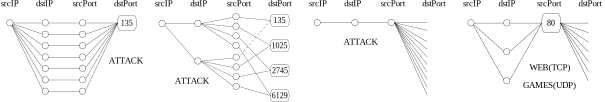
\includegraphics[width=0.9\linewidth]{figures/paper-encrypted/graphlets}
        \caption{A Visual Representation of Transport-Layer Interactions for Various Applications \cite{Karagiannis-2005-BLINC}.}
        \label{fig:graphlets}
    \end{center}
\end{figure}

Karagiannis et al.~\cite{Karagiannis-2005-BLINC} focused on host-based classification. Their method uses only information from the network level and therefore is not affected by transport layer encryption (e.g., TLS). The authors classified the behaviour of the hosts on social, functional, and application levels without access to packet payloads or headers. Each level was classified independently, and a cross-level classification was performed afterwards. Particular applications were represented using graphlets, see Figure~\ref{fig:graphlets}, which are representations of the application’s behaviour. The authors then used heuristics to refine the classification. The ground truth for captured datasets was established by using a signature-based payload classification. Without using transport layer information, only the following traffic classes were identified: web, p2p, data (FTP, database), network management (DNS, SNMP, NTP), mail (SMTP, POP, IMAP), news (NNTP), chat (IRC, AIM, MSN messenger), streaming, and gaming.
% INPUT: Host community, Host, Flow (transport protocol, avg packet size)
% TECHNIQUE: basic statistical, graphlets, heuristics
% OUTPUT: host->application type
% dataset: custom, real
% partial flow: no

Wright et al.~\cite{Wright-2006-Inferring} worked on classification of traffic in encrypted tunnels. Multiple flows can be wrapped in a single flow representing the encrypted tunnel. The information from the packet headers was not applicable; therefore the authors used only packet sizes, timing, and communication direction. A $k$-nearest neighbour classifier was used for classification when all TCP connections in a set carried the same application protocol. When TCP connections carried different application protocols, the authors used Hidden Markov Models. The authors also demonstrated that it is possible to determine the number of flows in an encrypted tunnel. The port numbers were used to obtain a ground truth for the captured dataset. The authors argue that mislabelled data only decreased the efficiency of their classification algorithm and therefore the real accuracy would be even higher than the reported one. The classifiers were able to detect the following application protocols: HTTP, HTTPS, SMTP, AIM, FTP, SSH, and Telnet.
% INPUT: flow
% TECHNIQUE: k-NN, HMM
% OUTPUT: flow->application protocol
% dataset: custom, real
% partial flow: no

Koch and Rodosek~\cite{Koch-2010-Command} proposed a system for detecting interactive attacks using SSH. Packet sizes, IP addresses, and packet inter-arrival times were used to create clusters of packets which were likely to match an SSH command and its corresponding response. The SSH protocol was recognised based on the port number, and individual commands were identified from the clusters. Following this, sequences of commands were evaluated, and possible malicious sequences were reported. The system allows for the customisation of malicious sequences' definitions using a sub-goals characterisation. Each sub-goal is mapped to a malicious event, such as data gathering or system manipulation. The results from the evaluation of the proposed method show that such identification is possible. 
% INPUT: Packet (packet size, inter-arrival times, IP addresses)
% TECHNIQUE: Statistical Method->[Basic Statical, Heuristics]
% OUTPUT: Fine-Grained (commands on SSH)
% dataset: unknown
% partial flow: yes

Khakpour and Liu~\cite{Khakpour-2013-Information} used an entropy of packet payloads for classifying traffic. The authors showed how to compute the entropy of files and how to modify the formula for on-the-fly computation. Several entropy values were computed for each packet. CART and support vector machine (SVM) methods were used for a subsequent classification based on the computed values. Their results demonstrated that SVM methods provide comparable accuracy with less false positives. The authors argue that it is necessary to exclude application layer headers such as HTTP response or picture headers. The reason for this is that computing entropy on the headers leads to bias and misclassification of a packet. Therefore, a cut-off threshold was used to strip application headers from unknown protocols. The traffic was first classified into three categories: text, encrypted, and binary. The authors also postulated that the classification can be more fine-grained and they investigated the classification of application protocols. Then, they demonstrated that it is possible to determine an encryption algorithm with higher accuracy than random guessing, which they found surprising.
% INPUT: Packet Payload
% TECHNIQUE: [Basic statistical (entropy), SVM, CART]
% OUTPUT: flow -> [application type (text, encrypted, binary), application protocol]
% dataset: private, artificial, real
% partial flow: no

\subsection{A Summary of Machine Learning and Statistical Encrypted Traffic Classification}\label{subsec:methods-summary}

We have provided a summarising overview of the feature-based traffic classification papers and methods they use in Table~\ref{tab:method_categories}. Where a method belongs to multiple categories, it is not marked as a hybrid, but all the categories are listed instead. We find this approach more descriptive than using a hybrid category as defined by the taxonomy.

\newcommand{\legendskip}{1.5cm}
\begin{sidewaystable}
    \centering
    \scriptsize
    \begin{varwidth}{\textheight}
    \renewcommand{\arraystretch}{1.1}
    \setlength{\tabcolsep}{0.6em} % less horizontal padding to fit to page
    \vfuzz=100pt % just get rid of those freaking warnings as an alternative to rewriting the whole table
    \begin{tabu}{c|[1pt] c|[1pt] l|l|l|l|l|[1pt] c|c|[1pt] l|l|l|l|l|l|l|l|[1pt] r @{$~\to~$} l|[1pt] c| c|[1pt] l|l|l|l|c}
        \multicolumn{1}{c|[1pt]}{} & \multicolumn{1}{c|[1pt]}{} & \multicolumn{5}{c|[1pt]}{} & \multicolumn{1}{c|}{} & \multicolumn{1}{c|[1pt]}{} & \multicolumn{8}{c|[1pt]}{} & \multicolumn{2}{c|[1pt]}{} & & \multicolumn{1}{c|[1pt]}{} & \multicolumn{5}{c}{} \\
                
        \multirow{3}{*}{\rotatebox[origin=r]{90}{\textbf{Reference}\hspace{38pt}}} & \multirow{3}{*}{\rotatebox[origin=r]{90}{\centering \textbf{Publication year}\hspace{13pt}}} & \multicolumn{5}{c|[1pt]}{\textbf{Input}} & \multirow{3}{*}{\rotatebox[origin=l]{90}{\textbf{Number of features}\hspace{7pt}}} & \multirow{3}{*}{\rotatebox[origin=l]{90}{\textbf{Feature selection}\hspace{17pt}}} & \multicolumn{8}{c|[1pt]}{\textbf{Technique}} & \multicolumn{2}{c|[1pt]}{\multirow{3}{*}{\textbf{Output}\vspace{23pt}}} & \multirow{3}{*}{\rotatebox[origin=l]{90}{\textbf{Encrypted proto. ident.}\hspace{-5pt}}} & \multirow{3}{*}{\rotatebox[origin=l]{90}{\textbf{Real-time ident.}\hspace{20pt}}} & \multicolumn{5}{c}{\multirow{2}{*}{\textbf{Dataset}\vspace{11pt}}}\\[0.10cm]
        
        \cline{3-7} \cline{10-17} \cline{22-26}
        
        \multicolumn{1}{c|[1pt]}{} & \multicolumn{1}{c|[1pt]}{} & \multirow{2}{*}{\rotatebox[origin=l]{90}{\textbf{Traf. Payload}\hspace{15pt}}} & \multicolumn{4}{c|[1pt]}{\textbf{Traf. Properties}\bigstrut} & \multicolumn{1}{c|}{} & \multicolumn{1}{c|[1pt]}{} & \multirow{2}{*}{\rotatebox[origin=r]{90}{\textbf{Payload Ins.}\hspace{14pt}}} &\multirow{2}{*}{\rotatebox[origin=r]{90}{\textbf{Graphlets}\hspace{22pt}}} & \multicolumn{2}{c|}{\textbf{Statis.}} &    \multicolumn{3}{c|}{\textbf{Machine}} & \multicolumn{1}{c|[1pt]}{\multirow{2}{*}{\textbf{Method(s)}\vspace{-33pt}}} & \multicolumn{2}{c|[1pt]}{} & & \multicolumn{1}{c|[1pt]}{} & \multirow{2}{*}{\rotatebox[origin=l]{90}{\textbf{Public}\hspace{40pt}}} & \multirow{2}{*}{\rotatebox[origin=l]{90}{\textbf{Private}\hspace{38pt}}} & \multirow{2}{*}{\rotatebox[origin=l]{90}{\textbf{Real}\hspace{47pt}}} & \multirow{2}{*}{\rotatebox[origin=l]{90}{\textbf{Artificial}\hspace{31pt}}} & \multirow{2}{*}{\parbox[c]{1.4cm}{\textbf{Ground truth}\vspace{-32pt}}} \\
        
        \cline{4-7} \cline{12-16}
        
        \multicolumn{1}{c|[1pt]}{} & \multicolumn{1}{c|[1pt]}{} & \multicolumn{1}{c|}{} & \rotatebox[origin=l]{90}{\textbf{Host Com.}\hspace{7pt}} & \rotatebox[origin=l]{90}{\textbf{Host}\hspace{1pt}} & \rotatebox[origin=l]{90}{\textbf{Flow}\hspace{1pt}} & \rotatebox[origin=l]{90}{\textbf{Packet}\hspace{1pt}} & \multicolumn{1}{c|}{} & \multicolumn{1}{c|[1pt]}{} & \multicolumn{1}{c|}{} & \multicolumn{1}{c|}{} & \rotatebox[origin=l]{90}{\textbf{Basic}} &    \rotatebox[origin=l]{90}{\textbf{Heuristic}} & \rotatebox[origin=l]{90}{\hspace{1pt}\textbf{Sup.}} & \rotatebox[origin=l]{90}{\textbf{Non Sup.}}    & \rotatebox[origin=l]{90}{\textbf{Semi Sup.}} & \multicolumn{1}{c|[1pt]}{} & \multicolumn{2}{c|[1pt]}{} & \multicolumn{1}{c|}{} & \multicolumn{1}{c|[1pt]}{} & \multicolumn{1}{c|}{} & \multicolumn{1}{c|}{} & \multicolumn{1}{c|}{} & \multicolumn{1}{c|}{}  \\
        \hline\hline
        \cite{DeMontigny-Leboeuf-2005-Flow}  & 2005  & & & & \cmark & \cmark         & $\subseteq$ 39 & \xmark  & & & \cmark & & & & &                                                                          & F & AP, AT  & \xmark  &         & & \cmark & \cmark &                        & port              \\ \hline
        \cite{Karagiannis-2005-BLINC}        & 2005  & & \cmark & \cmark & \cmark &  & -- & \xmark              & & \cmark & \cmark & \cmark & & & &                                                            & H & AT      & \cmark  &         & & \cmark & \cmark &                        & signature         \\ \hline
        \cite{Wright-2006-Inferring}         & 2006  & & & & \cmark & \cmark         & 3 & \xmark               & & & & & \cmark & & \cmark & HMM, $k$-nearest neighbor                                         & F & AP      & \cmark  &         & & \cmark & \cmark &                        & port              \\ \hline
        \cite{Bernaille-2007-Early}          & 2007  & & & & & \cmark                & 3 & \xmark               & & & & & & & \cmark & Gaussian Mixture Model                                                   & P & AP      & \cmark  & \cmark  &  & \cmark & \cmark &                       & signature, known  \\ \hline
        \cite{Alshammari-2007-flow}          & 2007  & & & & \cmark &                & 22 & \xmark              & & & & & \cmark & & & AdaBoost, RIPPER                                                         & F & AT      & \cmark  &         & \cmark & \cmark & \multicolumn{2}{c|}{--}  & port, known       \\ \hline
        \cite{Maiolini-2009-Real}            & 2009  & & & & & \cmark                & 3 & \xmark               & & & & & & & \cmark & $k$-means                                                                & F & AP      & \cmark  & \cmark  & & \cmark & & \cmark                        & known             \\ \hline
        \cite{Alshammari-2009-Machine}       & 2009  & & & & \cmark &                & 22 & \xmark              & & & & & \cmark & & & \parbox[c]{2.4cm}{AdaBoost, RIPPER, SVM,\\ Naive Bayes, C4.5}\bigstrut   & F & AP      & \xmark  &         & \cmark & \cmark & \cmark &                 & port, signature   \\ \hline
        \cite{Alshammari-2009-Preliminary}   & 2009  & & & & \cmark & \cmark         & $\subseteq$ 30 & \xmark  & & & & & \cmark & & & RIPPER, C4.5                                                             & F & AT      & \xmark  &         & & \cmark & \cmark & \cmark                 & signature, known  \\ \hline
        \cite{Alshammari-2009-Classifying}   & 2009  & & & & & \cmark                & 39 & \cmark              & & & & & \cmark & & & AdaBoost, C4.5, Genetic Programming        & F & AP      & \xmark  &         & & \cmark & \cmark &                        & signature, port   \\ \hline
        \cite{Bacquet-2009-Investigation}    & 2009  & & & & \cmark &                & 38 & \cmark              & & & & & & & \cmark & $k$-means, Genetic Programming                                           & F & AP      & \xmark  &         & & \cmark & \cmark &                        & signature         \\ \hline
        \cite{Alshammari-2010-Investigation} & 2010  & & & & \cmark & \cmark         & 22 & \xmark              & & & & & \cmark & & & AdaBoost, C4.5, Genetic Programming        & F & AP      & \cmark  &         & & \cmark & \cmark & \cmark                 & signature, known  \\ \hline
        \cite{BarYanai-2010-Realtime}        & 2010  & & & & \cmark &                & 17 & \xmark              & & & & & & & \cmark & $k$-nearest neighbor, $k$-means                                          & F & AP      & \xmark  & \cmark  & & \cmark & \cmark &                        & signature, known  \\ \hline
        \cite{Sun-2010-Novel}                & 2010  & \cmark & & & \cmark &         & 6 & \xmark               & \cmark & & & & \cmark & & & Naive Bayes                                                       & F & AP      & \cmark  &         & \cmark & \cmark & \cmark &                 & known             \\ \hline
        \cite{Koch-2010-Command}             & 2010  & & & & & \cmark                & -- & \xmark              & & & \cmark & \cmark & & & &                                                                   & F & FG      & \xmark  & \cmark  & \multicolumn{4}{c|}{--}                    & --                \\ \hline
        \cite{Bacquet-2011-Genetic}          & 2011  & & & & \cmark &                & 38 & \cmark              & & & & & & & \cmark & (hierarchical) $k$-means                                                 & F & AP      & \xmark  &         & & \cmark & \cmark &                        & signature         \\ \hline
        \cite{Wang-2011-Using}               & 2011  & \cmark & & & &                & 7 & \cmark               & & & \cmark & & & & & Entropy                                                                  & F & AT      & \cmark  & \cmark  & & \cmark & & \cmark                        & known             \\ \hline
        \cite{Okada-2011-Application}        & 2011  & & & & \cmark &                & 49 & \cmark              & & & & & \cmark & & & Naive Bayes                                                              & F & AP      & \cmark  &         & & \cmark & & \cmark                        & known             \\ \hline
        \cite{Arndt-2011-Comparison}         & 2011  & & & & \cmark &                & $\subseteq$ 46 & \cmark  & & & & & \cmark & & & C4.5, $k$-means, MOGA                                                    & F & AP      & \xmark  &         & \cmark & \cmark & \cmark &                 & signature, port   \\ \hline
        \cite{Alshammari-2011-Can}           & 2011  & & & & \cmark & \cmark         & 61 & \cmark              & & & & & \cmark & & & AdaBoost, C4.5, Genetic Programming        & F & TP      & \xmark  &         & \cmark & \cmark & \cmark &                 & signature, port   \\ \hline
        \cite{Korczynski-2012-Classifying}   & 2012  & & & & \cmark &                & 9 & \cmark               & & & \cmark & & & & & Statistical Protocol Identification                                      & F & AP      & \cmark  &         & & \cmark & & \cmark                        & known             \\ \hline
        \cite{Zhang-2013-Encrypted}          & 2013  & & & & \cmark &                & 22 & \xmark              & & & & & & & \cmark & $k$-means                                                                & F & AP      & \xmark  &         & \cmark & \cmark & \cmark &                 & signature         \\ \hline
        \cite{Du-2013-Design}                & 2013  & & & & \cmark & \cmark         & 7 & \xmark               & & & & & & & \cmark & $k$-means                                                                & F & AS      & \xmark  &         & & \cmark & & \cmark                        & known             \\ \hline
        \cite{Khakpour-2013-Information}     & 2013  & \cmark & & & &                & 10 & \cmark              & & & \cmark & & \cmark & & & Entropy, SVM, CART                                                & F & AT, AP  & \cmark  &         & & \cmark & \cmark & \cmark                 & known             \\ \hline
        \cite{Amoli-2013-real}               & 2013  & & & & \cmark & \cmark         & 23 & \xmark              & & & \cmark & & & \cmark & & Change point detection, Clustering  & F & A       & \xmark  &         & \multicolumn{4}{c|}{--}                    & --                \\ \hline
        \cite{Kumano-2014-Towards}           & 2014  & & & & \cmark &                & 29 & \cmark              & & & & & \cmark & & & C4.5, SVM                                                                & F & AT      & \cmark  & \cmark  & & \cmark & & \cmark                        & known             \\ \hline
        \cite{Korczynski-2014-Markov}        & 2014  & \cmark & & & & \cmark         & -- & \xmark              & & & \cmark & & & & & Markov chains                                                            & F & AP      & \cmark  &         & & \cmark & \cmark &                        & signature         \\ \hline
    \end{tabu}
    \renewcommand{\arraystretch}{1.000}
    \begin{center}
    \begin{tabular}{lll@{\hskip \legendskip}ll@{\hskip \legendskip}ll@{\hskip \legendskip}ll}
%         &&&&&&&& \\
        \multirow{2}{*}{\textbf{Output column legend:}\hspace{20pt}} & A & Anomaly & AP & Application Protocol & AS & Application Software & T & Application Type \\
        & H & Host & F & Flow & FG & Fine-Grained & TP & Traffic Payload \\
%         &&&&&&&& 
    \end{tabular}
    \end{center}
    \end{varwidth}
    \caption{A Summary Table of Cited Papers and Methods They Use to Detect Encrypted Traffic.}
    \label{tab:method_categories}
\end{sidewaystable}

Most of the surveyed methods use flow or packet header features as an input for the classification techniques. The authors of~\cite{Alshammari-2009-Preliminary, Alshammari-2011-Can} compare the results gained by utilising packet header features and flow features. They show that using both sets of features can result in faster and more accurate classification algorithms. Nevertheless, using all the available traffic features does not necessarily lead to the best classification performance as demonstrated by the authors of~\cite{Alshammari-2009-Classifying}.

The column \emph{Number of features} shows how many flow or packet header features were used in each method. Some methods used different subsets of the features for different algorithms, and this is denoted by the $\subseteq$ mark. Moreover, some of the methods used a feature selection algorithm to select the best combination of features from the entire feature set. These methods are marked in the \emph{Feature selection} column. For this case, the \emph{Number of features} column represents the initial number of features.

Most classification algorithms are based on machine learning. The category of supervised machine learning algorithms is represented by Hidden Markov Models, RIPPER, AdaBoost, Support Vector Machines, C4.5, and Naive Bayes. Several works~\cite{Alshammari-2007-flow, Alshammari-2009-Machine, Alshammari-2010-Investigation, Alshammari-2011-Can} compare these algorithms to establish which is the best for the task of classifying traffic. The C4.5 algorithm performs the best in several cases; however, genetic programming is reported to achieve the best results in~\cite{Alshammari-2011-Can}. The second most common algorithm category is the semi-supervised machine learning, which is dominated by clustering algorithms. The $k$-means algorithm is the most frequent in this category, and the $k$-nearest neighbour comes second. The popularity of $k$-means is due to its variability, which allows it to be fine-tuned for various purposes. It is often combined with genetic algorithms to find the best setting. The authors of~\cite{Wang-2011-Using, Khakpour-2013-Information} use the entropy of packet payloads to classify traffic. Using simple statistical properties of the traffic is the third most common classification method. Other methods are rarely used, mainly because they cannot learn from labelled traffic and therefore require too much effort to set up.

The SSH protocol is heavily used as a classification example. The authors of~\cite{Alshammari-2009-Classifying, Alshammari-2007-flow, Alshammari-2009-Preliminary, Alshammari-2009-Machine, Alshammari-2011-Can, Arndt-2011-Comparison, Bacquet-2009-Investigation, Bacquet-2011-Genetic, Zhang-2013-Encrypted} test their methods for recognising SSH and non-SSH traffic. Maiolini et al.~\cite{Maiolini-2009-Real} take the classification one step further and identify the type of traffic encapsulated in an SSH connection. The authors of~\cite{Bernaille-2007-Early, Korczynski-2014-Markov, Sun-2010-Novel} use SSL/TLS traffic and identify underlying application protocols. Since the SSL/TLS protocol is more general and is used to encrypt various types of traffic, the complexity of identification is higher than for SSH. Another very popular protocol for identification is Skype, which is addressed by the authors of~\cite{Alshammari-2009-Machine, Alshammari-2011-Can, Korczynski-2012-Classifying, Korczynski-2014-Markov}.

Some of the methods focus only on identifying encrypted traffic, whereas others try to identify the underlying application protocol. The methods which perform a more thorough analysis to gain information about the application protocol are indicated in the column \emph{Encrypted protocol identification.}

Because all methods, with the exception of~\cite{Karagiannis-2005-BLINC}, classify whole flows and rely mostly on flow features, they are rarely able to classify traffic in real-time. However, the authors of~\cite{BarYanai-2010-Realtime, Bernaille-2007-Early, Kumano-2014-Towards, Maiolini-2009-Real, Wang-2011-Using} achieved near real-time classification by extracting features of only a fixed number of packets in a flow. They argue that the first packets carry enough information for classification. Using a higher number of packets increases accuracy; therefore it is possible to strike a balance between accuracy and early identification.

The \emph{Dataset} columns describe whether the data used to evaluate the presented methods was taken from a live network (Real) or generated by a tool (Artificial). We also identify if the datasets were publicly available (Public), were made available by the authors (Published), or kept undisclosed as they contain sensitive information (Private). If more than one dataset was used for each evaluation, we simply performed a union of the dataset descriptions. The \emph{Ground truth} column indicates how the ground truth was obtained for each dataset. Common methods are based on port numbers or signatures, which use the packet payload. When the datasets are generated manually, the ground truth is known in advance.

The classification accuracy reported by authors of the surveyed methods depends heavily on the used datasets. All authors use their own private datasets, which are seldom published. Such methods simply cannot be compared without repeating the experiments on a common dataset. The authors of~\cite{Alshammari-2007-flow, Alshammari-2009-Machine, Alshammari-2011-Can, Arndt-2011-Comparison, Sun-2010-Novel, Zhang-2013-Encrypted} also used publicly available datasets which were either labelled beforehand, using payload when available, or simply labelled using port numbers. A combination of datasets is often used to test the robustness of the methods. 

The surveyed methods show that a lot of effort was put into classifying encrypted traffic. We believe that there are several points that should be taken into account in any future research in this field. First, identifying encrypted traffic is not enough. The identification of the underlying protocol is the real challenge. Second, an SSL/TLS protocol should be used as the reference protocol, as it can contain much more complex traffic than the SSH protocol. Finally, the used traces should be labelled and made available to other researchers. Following these points does not limit the scope of future research; however, it simplifies the comparison of the presented approaches and allows others to verify the results more easily.


%%%%%%%%%%%%%%%%%%%%%%%%%%%%%%%%%%%%%%%% CONCLUSIONS %%%%%%%%%%%%%%%%%%%%%%%%%%%%%%%%%%%%%%%%%%%%%%%%%%%%%%%%%%%%%


\section{Conclusions} \label{sec:enc-conclusions}

In this chapter, we presented an overview of current approaches for the classification and analysis of encrypted traffic. First, we selected a number of the most widely used encryption protocols and described their packet structure and standard behaviour in a network. Second, we focused on information which is provided by encryption protocols themselves. We found that the initiation phase often provides information about the protocol version, ciphers used, and the identity of at least one communicating party. Such information can be used to monitor and enforce security policies in an organisation. We also discovered that the use of information from the unencrypted parts of an encrypted connection for a network anomaly detection is only briefly investigated by researchers. Information about communicating parties can be leveraged to discern the type of encrypted traffic. For example, the list of supported cipher suites provided by a client when establishing a secure connection can help to identify the client. We believe that the use of unencrypted parts from the initiation of an encrypted connection should be explored in more detail.

Before starting the analysis of the encrypted network traffic, it is necessary to identify it. Thus, we surveyed approaches to classifying network traffic. There are payload-based methods, which use knowledge of a packets' structure, and feature-based methods, which use characteristics specific to the protocol flow. For the payload-based classification, there are several open-source traffic classifiers which can identify encrypted traffic using pattern matching. The initiation of communication often has a strictly defined structure; therefore, the patterns can be constructed for specific protocols. The main difference between various classifiers is that some of them require traffic from both directions of the communication to correctly classify the flows.

Feature-based traffic classifiers have been intensively researched over the last decade. Many statistical and machine-based learning methods have been applied to the task of traffic classification. Despite this, there are no conclusive results to show which method has the best properties. The main reason is that the results depend heavily on the datasets used and the configuration of the methods. We have applied the multilevel taxonomy of Khalife et al.~\cite{Khalife-2014-multilevel} and categorised the existing methods. Our results show that most of the authors use private datasets, sometimes in combination with public ones. For this reason, the individual results are not directly comparable. Most of the methods use supervised or semi-supervised machine learning algorithms to classify flows and even determine the application protocol of a given flow. Most methods target encryption protocols, such as SSH, SSL/TLS, and encrypted BitTorrent, and use similar methods. However, there are also some novel works which apply innovative approaches to refine the classification up to deriving the content of the encrypted connections.

Most authors of feature-based classification methods claim that their approach is privacy sensitive as it does not require the traffic payload. However, privacy issues are much wider. In 2013, the Cyber-security Research Ethics Dialog \& Strategy Workshop~\cite{CAIDA-2013-Cyber} started a discussion about the influence of cyber-security research on the privacy of Internet users. Researchers need to keep in mind that their research activities have a significant impact on infrastructure security, network neutrality, and privacy of end users. 

In the past, internet protocols were not, or could not be, designed with security considerations in mind. The recent interest in privacy has motivated the IETF to reconsider this approach and discuss the privacy aspects of the protocols. Discussions held in~\cite{IETF-2014-IETF} revealed that monitoring privacy issues are of great concern. This discussion resulted in a new RFC~\cite{rfc7258}, where the IETF clearly states that pervasive monitoring is considered to be an attack. The document suggests that the IETF's protocols should be hardened against such monitoring. It is clear that the struggle between the demand for privacy and the need for security is still in the beginning.

